\documentclass[fleqn]{homework}

\student{Stephen Brennan (smb196)}
\course{EECS 477}
\assignment{Homework 4}
\duedate{October 30, 2015}

\usepackage{algpseudocode}
\usepackage{mathtools}
\usepackage{graphicx}
\usepackage{enumerate}

\begin{document}
  \maketitle

  \begin{problem}{1}
    \begin{question}
      To provide adequate medical service to its constituents at a reasonable
      cost, hospital administrators must constantly seek ways to hold staff
      levels as low as possible while maintaining sufficient staffing to provide
      satisfactory levels of health care.  An urban hospital has three
      departments: the emergency room (department 1), the neonatal intensive
      care nursery (department 2), and the orthopedics (department 3). The
      hospital has three work shifts, each with different levels of necessary
      staffing for nurses. The hospital would like to identify the minimum
      number of nurses required to meet the following three constraints:

      \begin{enumerate}[a.]
      \item The hospital must allocate at least 13, 32, and 22 nurses to the
        three departments over all shifts,
      \item The hospital must assign at least 26, 24, and 19 nurses to the three
        shifts over all departments, and
      \item The minimum and maximum number of nurses allocated to each
        department in a specific shift must satisfy the following limits:

        \begin{tabular}{|l|ccc|}
          \hline
          & Department 1 & Department 2 & Department 3 \\
          \hline
          Shift 1 & (6, 8) & (11, 12) & (7, 12) \\
          Shift 2 & (4, 6) & (11, 12) & (7, 12) \\
          Shift 3 & (2, 4) & (10, 12) & (5, 7) \\
          \hline
        \end{tabular}
      \end{enumerate}

      Suggest a method using maximum flows to identify the minimum number of
      nurses required to satisfy all the constraints.
    \end{question}

    For the purposes of notation, let $D(i)$ and $S(j)$ be the minimum numbers
    of nurses for department $i$ or shift $j$ respectively.  Let $MinDS(i,j)$
    and $MaxDS(i,j)$ be the minimum and maximum required amount of nurses for
    the pair of department $i$ and shift $j$.

    For intuition of this problem, we start by assuming that each pair of
    department and shift are given the maximum number of nurses.  The total flow
    will be the number of nurses we can remove while still satisfying each
    constraint.  To this end, we define nodes in a similar fashion to the matrix
    rounding problem presented in class.  For each pair of department $i$ and
    shift $j$, we create a node $a_{ij}$.  For each department $i$ we create a
    node $d_i$, and for each shift $j$ we create a node $s_j$.  Then, we create
    a source node $s$ and a sink node $t$.

    We create edges from $s$ to each $s_j$.  The lower bounds of these nodes
    will be 0, and the upper bounds will be the number of nurses we could remove
    in total from that shift.  This can be expressed as
    $\left(\sum_i MaxDS(i,j)\right) - S(j)$.  These upper bounds satisfy the
    constraints in (a).

    Next, for each pair $(i,j)$, we create an edge from $s_j$ to $a_{ij}$, and
    from $a_{ij}$ to $d_i$.  These edges will both have lower bound of 0, and
    upper bound $MaxDS(i,j) - MinDS(i,j)$.  These edges represent the number of
    nurses we could remove from each (department, shift) pairing, while still
    satisfying the constraints in (c).

    Finally, we create an edge from each $d_i$ to $t$.  These will have a lower
    bound of 0 and an upper bound of $\left(\sum_j MaxDS(i,j)\right) - D(i)$.
    These edges represent the number of nurses we could remove from each shift
    while satisfying the constraints in (b).

    The maximum flow solution will determine the maximum number of nurses that
    can be removed from the schedule in total.  In order to recover the amount
    of nurses assigned to each (department, shift) pairing, we simply need to
    translate from ``number of nurses removed'' to number of nurses assigned.
    This can be achieved by $MaxDS(i,j) -$ flow through $a_{ij}$.
  \end{problem}

  \begin{problem}{2}
    \begin{question}
      Formulate the contractor problem (Homework Assignment 1, problem 7) as a
      minimum cost network flow problem, write its dual and complementary
      slackness conditions, and prove that this problem has always an integer
      optimal solution.
    \end{question}

    As in previous assignments, I will use the notation that there are $n$
    contractors, the first $r$ of which are experienced.  Additionally, there
    will be $k$ locations.

    In the minimum cost network flow formulation of this problem, there will be
    a node for each contractor ($v_1, v_2, \dots, v_n$).  Each node $v_i$ will
    have supply $u_i$.  Furthermore, there will be two nodes for each location
    $j$---one for the required experienced contractor ($w_j$) and one for the
    rest of the contractors ($z_j$).  Each $w_J$ will have supply $-1$, and each
    $z_j$ will have supply $1-r_j$.

    Since there is no guarantee that the total number of contractors is equal to
    the total number of required contractors (only that there are at least that
    much, for the problem to be feasible), we must create a slack node $s$ with
    demand of $\sum_{i=1}^n u_i$ - $\sum_{j=1}^k r_j$.

    For each contractor $i$, there will be two types of edges:
    
    \begin{itemize}
    \item $(v_i, z_j)$, also with cost $c_{ij}$, $\forall j$.  The flow across
      these arcs will be labeled $x_{ij}$.
    \item $(v_i, s)$, with cost zero.  The flow across these arcs will be
      labeled $t_i$.
    \end{itemize}

    For experienced contractors $i \in [r+1,n]$, there will be an additional
    edge $(v_i, w_j)$, with cost $c_{ij}$, $\forall j$.  The flow across these
    arcs will be labeled $y_{ij}$.

    All edges in the network have 0 lower bound and $\infty$ upper bound.  This
    problem can therefore be expressed with the linear program:

    \begin{alignat*}{5}
      \min \sum_{i=1}^n \sum_{j=1}^k c_{ij} x_{ij} + \sum_{i=1}^r \sum_{j=1}^k c_{ij} y_{ij} & \text{ s.t.} \\
      t_i + \sum_{j=1}^k (x_{ij} + y_{ij}) &= u_i, && 1 \le i \le r && (\pi_i)\\
      t_i + \sum_{j=1}^k x_{ij} &= u_i,   &&r+1 \le i \le n \:\:  && (\pi_i)\\
      \sum_{i=1}^n x_{ij} &= r_j - 1,  && 1 \le j \le k && (\lambda_j)\\
      \sum_{i=1}^r y_{ij} &= 1, && 1 \le j \le k && (\gamma_j)\\
      \sum_{i=1}^n t_i &= \sum_{i=1}^n u_i - \sum_{j=1}^k r_i  && && (\eta)\\
      t_i, x_{ij}, y_{ij} &\ge 0  &&\\
    \end{alignat*}

    Since there are no arc upper bounds, there are no $\alpha_{ij}$ variables.
    I've given each type of node's mass balance constraint its own variable
    letter, instead of trying to decipher them using some subscript notation.

    The dual can therefore be mechanically produced:

    \begin{alignat*}{5}
      \max \sum_{i=1}^n \pi_i u_i + \sum_{j=1}^k (r_j-1) \lambda_j + \sum_{j=1}^k \gamma_j + &\eta \left(\sum_{i=1}^n u_i - \sum_{j=1}^k r_i\right), \text{ s.t.} \\
      \pi_i + \eta &\le 0, && \:\: 1 \le i \le n, \:\: && (t_i) \\
      \pi_i + \lambda_j &\le c_{ij} && \:\: \forall i,j, \:\: && (x_{ij}) \\
      \pi_i + \gamma_j &\le c_{ij} && \:\: 1 \le i \le r, \forall j, \:\: && (y_{ij}) \\
      \pi_i, \lambda_j, \gamma_j, \eta &\text{ unconstrained}
    \end{alignat*}

    The complementary slackness conditions:

    \begin{align*}
      t_i(\pi_i + \eta) &= 0 \\
      x_{ij} (c_{ij} - \pi_i - \lambda_j) &= 0 \\
      y_{ij} (c_{ij} - \pi_i - \gamma_j) &= 0 \\
    \end{align*}

    I could continue listing the corresponding ones from the primal, but since
    all constraints are equality in the primal, they are trivially true and not
    particularly interesting.

    To prove that the solutions to this problem are linear, it is suffucient to
    note that MCNF is a unimodular problem, and since the $b_i$ values (i.e.,
    $u_i$ and $r_j$) must all be integers, all solutions to the contractor
    problem must be integer
  \end{problem}

  \begin{problem}{3}
    \begin{question}
      Let $G=(V, E)$ be a directed graph with lengths $w(e)$ associated to each
      arc $e \in E$, and let $s \in V$ be a vertex. Recall that
      $d(v) \le d(u) + w(u,v)$ for $(u,v) \in E$ by linear programming duality,
      where $d(u)$ is the distance of $u \in V$ from $s$. Show that the
      following invariant holds during the execution of Dijkstra's algorithm: if
      $S$ is the set of permanently labeled nodes and $d(u)$ is the current
      label of vertex $u$, then $d(v) \le d(u) + w(u,v)$ for $(u,v) \in E$,
      $u \in S$, $v \not\in S$.
    \end{question}

    Consider the following definition of Dijkstra's algorithm, from CLRS:

    \begin{algorithmic}
      \Function{Dijkstra}{$G, w, s$}
        \State $S \gets \emptyset$
        \State $Q \gets G.V$
        \While{$Q \ne \emptyset$}
          \State $u \gets$ Extract-Min$(Q)$
          \State $S \gets S \cup \{u\}$
          \For{$v\in G.V: \:\: (u,v) \in G.E$}
            \If{$d(v) > d(u) + w(u,v)$}
              \State $d(v) \gets d(u) + w(u,v)$
              \State $v.\pi \gets u$  \Comment{ records the predecessor node}
            \EndIf
          \EndFor
        \EndWhile
      \EndFunction
    \end{algorithmic}

    \begin{itemize}
    \item \textbf{Initialization:} Since $S$ is initialized to $\emptyset$, the
      condition is vacuously true on initialization of the loop.
    \item \textbf{Maintenance:} Assume that the invariant is true at the
      beginning of the while loop.  Each iteration of the outer loop, a node $u$
      is selected from $V \setminus S$ and added to $S$.  We must first show
      that the invariant is true for $u$ and all $v\in V\setminus S$ at the end
      of the loop.  If the invariant were false for any $v$ before the for loop,
      then the inner if statement would have assigned
      $d(v) \gets d(u) + w(u,v)$, thus satisfying the invariant.  So, the
      invariant must be true between $u$ and all $v \in V \setminus S$.

      We must also show that the condition has not been violated for any $t$
      that was in $S$ at the beginning of the loop.  Since $d(v)$ was only
      decreased for $v \in V \setminus S$, the condition could not have been
      violated during the execution of the loop.  Thus, the invariant is
      maintained.
    \end{itemize}

    (No termination step is necessary, since we only are proving that the
    invariant holds, not that a property results due to the invariant.)
  \end{problem}

  \begin{problem}{5}
    \begin{question}
      Apply the successive shortest paths algorithm to the minimum cost flow
      problem in the figure. Show that the algorithm performs eight
      augmentations of unit flow and that their cost (i.e., the sum of the arc
      costs in the path in the residual network) is 0, 1, 2, 3, 4, 5, and 6.

      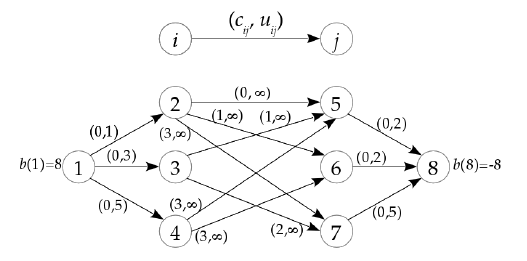
\includegraphics[width=0.6\textwidth]{p5-fig.png}
    \end{question}

    We start with the original residual, with $\pi=x=0$.  Note that in all
    diagrams, arcs are labeled by $(c_{ij}^\pi, u_{ij})$.

    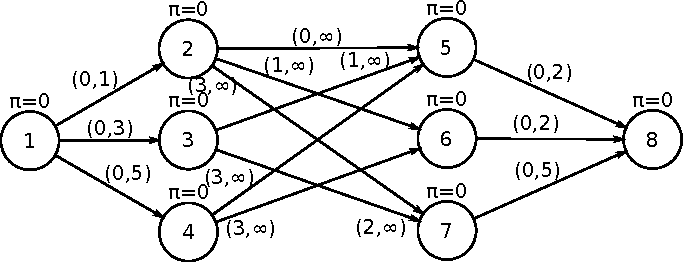
\includegraphics{p5-00-initial.pdf}

    Next, we update the values of $\pi$ and $c_{ij}^\pi$, and find the shortest
    path.

    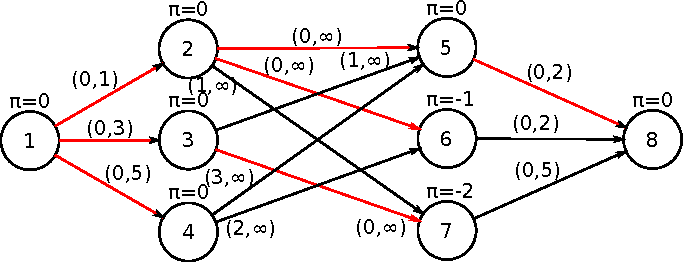
\includegraphics{p5-01-update-pi.pdf}

    Now, we augment by sending one unit of flow from 1 to 2 to 5 to 8:

    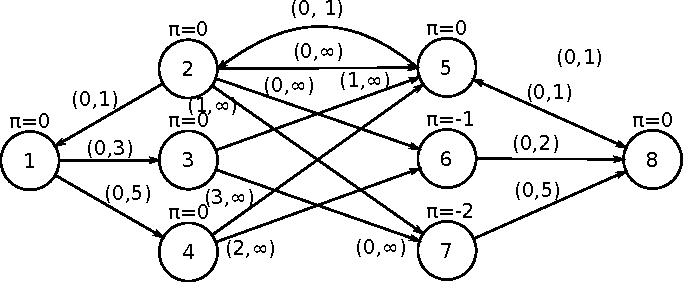
\includegraphics{p5-02-augment.pdf}

    Again, we update the values of $\pi$ and $c_{ij}^\pi$, and find the shortest
    path.

    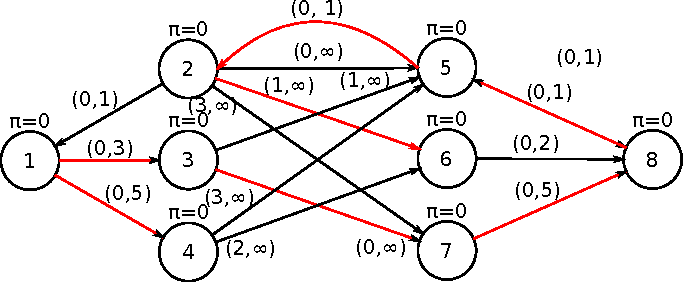
\includegraphics{p5-03-update-pi.pdf}

    Next, we augment by sending three units of flow from 1 to 3 to 7 to 8.

    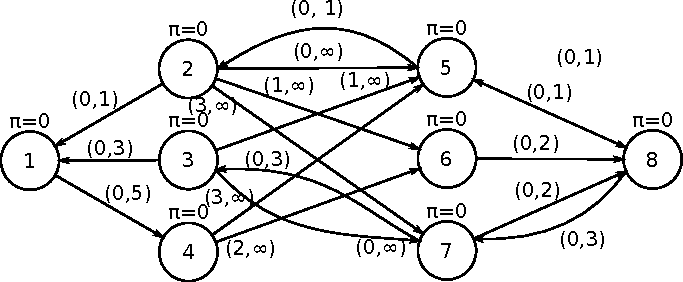
\includegraphics{p5-04-augment.pdf}

    Again, update $\pi$ and $c_{ij}^\pi$, and find the shortest path:

    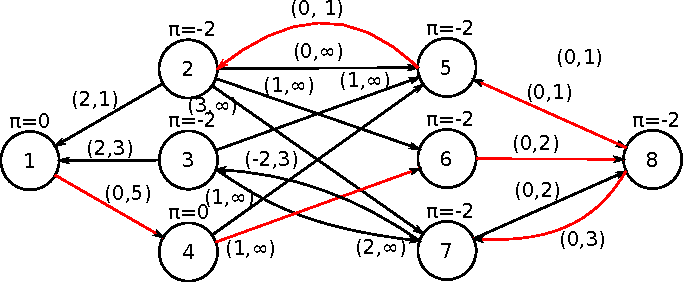
\includegraphics{p5-05-update-pi.pdf}

    Unfortunately, from here we have negative edge weights, meaning I probably
    have done something wrong.  Especially considering that the last
    augmentation sent 3 units of flow instead of 1.
  \end{problem}

  \begin{problem}{7}
    \begin{question}
      Consider the following practical improvement of the successive shortest
      path algorithm:

      \begin{enumerate}[a.]
      \item Terminate the execution of Dijkstra's algorithm whenever it
        permanently labels a deficit node $v$, and

      \item Modify the node potentials by setting $\pi(u)$ to $\pi(u)-d(u)$ if
        node $u$ is permanently labelled and by setting $\pi(u)$ to
        $\pi(u)-d(v)$ if node $u$ is temporarily labelled.
      \end{enumerate}

      Show that after the algorithm has updated the node potentials in this
      manner, all the arcs in the residual network have non-negative reduced
      costs and that all arcs in the shortest path from node $k$ to node $v$
      have zero reduced cost. Use the statement of problem 3.
    \end{question}
  \end{problem}

\end{document}